% !TEX TS-program = xelatex
% !TEX encoding = UTF-8 Unicode

% This is a simple template for a LaTeX document using the "article" class.
% See "book", "report", "letter" for other types of document.

\documentclass[11pt]{article}

\usepackage[margin=1in]{geometry}
\usepackage{fancyhdr}

\usepackage{parskip}
\usepackage{framed}
\usepackage{amsmath,amsthm,amssymb}

\newtheorem*{conjecture}{Conjecture}

\usepackage{titlesec}

\usepackage[svgnames]{xcolor}

%\usepackage{enumerate}
\usepackage{enumitem}
\newcounter{descriptcount}


%\usepackage{mathpazo}
\usepackage{mathtools}
\usepackage{unicode-math}
\usepackage{empheq}
\usepackage[most]{tcolorbox}
\usepackage{cancel}

\usepackage{caption}

\usepackage{xunicode} %handle unicode
\usepackage{xltxtra} %XeTeX extras
\usepackage{fontspec} %use OTF/TTF fonts

%\newcommand{\lmr}{\fontfamily{lmr}\selectfont} % Latin Modern Roman


%\setmainfont{Myriad Pro} %use this font
%\setmathfont{Adobe Garamond Pro} %use this font for math

\titleformat{\section}
  {\large\bf}{\thesection}{0.25em}{}[\titlerule]
\titlespacing{\section}
  {0pt}{*1.5}{0.25em}

\titleformat{\subsection}
  {\normalfont\bf}{\thesubsection}{0.25em}{}
\titlespacing{\subsection}
  {0pt}{*1}{0.125em}

\renewcommand\thesection{\Alph{section}.}
\renewcommand\thesubsection{\thesection\arabic{subsection}}
\renewcommand\thesubsubsection{(\roman{subsubsection}).}

\renewcommand{\labelitemi}{\textemdash}

\DeclareMathOperator{\dif}{d\!}
%\DeclareMathOperator{\Pr}{P}
\DeclareMathOperator{\E}{E}
\DeclareMathOperator{\Cov}{Cov}
\DeclareMathOperator{\var}{var}
\DeclareMathOperator{\F}{\mathfrak{F}}
\DeclareMathOperator{\Poisson}{Poisson}
\DeclareMathOperator{\Bernoulli}{Bernoulli}
\DeclareMathOperator{\Binomial}{Binomial}
\DeclareMathOperator{\Order}{O}
\DeclareMathOperator{\Uniform}{Uniform}
\DeclareMathOperator*{\argmax}{argmax}
\DeclareMathOperator{\Tr}{Tr}
\DeclareMathOperator{\diag}{diag}
\DeclareMathOperator{\KLsym}{KL}
\DeclarePairedDelimiterX{\klx}[2]{(}{)}{%
  #1\,\delimsize\|\,#2%
}
\newcommand{\KL}{\KLsym\klx}

\newcommand{\logdet}[1]{\log \left| {#1} \right| }

\newcommand{\xb}{\mathbf{x}}
\newcommand{\zb}{\mathbf{z}}
\newcommand{\ub}{\symbf{\mu}}
\newcommand{\Sb}{\symbf{\Sigma}}
\newcommand{\Wb}{\mathbf{W}}

\newcommand*{\tran}{^{\mkern-1.5mu\mathsf{T}}}
\newcommand*{\invtran}{^{\mkern-1.5mu\mathsf{-T}}}


\newenvironment{propertybox}{%
   \def\FrameCommand{\colorbox{LightSteelBlue}}%
   \MakeFramed{\advance\hsize-\width \FrameRestore}}
 {\endMakeFramed}

\lhead{\textbf{ELEC548}}
\chead{Dimensionality Reduction}
\cfoot{}
\rhead{}
\rfoot{\thepage}
\pagestyle{fancyplain}

%\setlength\parindent{0pt}

\allowdisplaybreaks


\begin{document}
\setmainfont{Myriad Pro} %use this font
%\setmathfont{Latin Modern Math}
%\setmathfont{TG Pagella Math}

\begin{center}
\large
\textbf{ELEC 548} Dimensionality Reduction
\end{center}

\textit{Dimensionality reduction} is a very useful tool for visualizing and
understanding data that are in a high dimensional space. If we assume that most
high dimensional data actually exist primarily in a lower dimensional space,
the extra dimensions are a form of noise. Thus, many other machine learning
problems, such as clustering, would be more robustly be performed in the lower
dimensional space. Dimensionality reduction tools allow us to estimate the
connection between higher dimensional data and lower dimensional
representations. A good reference for this topic is Chapter 12 of Bishop's
\textit{Pattern Recognition and Machine Learning}.

\section{Principal Components Analysis}
\begin{align*}
  \text{\underline{Data set}:} & \; \xb_n \in \mathbb{R}^D, \, n = 1, \ldots, N \\
  \text{\underline{Goal:}} & \; \text{Project data into a space with
  dimensionalty $M < D$ while} \\
  & \; \text{maximizing the variance of the projected data.}
\end{align*}

\textit{Intution: Why do we want to maximize the variance?} Imagine the corner case that in one
dimension of our data $i$, there is no variability at all (the $\xb_n^{(i)}$ are
equal for all i). Then, that dimension is not particularly useful and could be
safely ignored as we look for interesting features. But in the new
$D-1$-dimensional data, the variance would be the same as in the original data
set (i.e., maximized for $M=D-1$).

Principal Components Analysis starts with the \textbf{sample covariance matrix},
$\mathbf{S}$.
\begin{equation*}
  \mathbf{S} \equiv \frac{1}{N} \sum_{n=1}^N (\xb_n - \ub) (\xb - \ub)\tran,\,
  \text{where } \ub = \frac{1}{N} \sum_{n=1}^N \xb_n
\end{equation*}

\subsection{Diagonalization / ``Eigendecomposition''}
Any covariance matrix (symmetric, positive semidefinite) can be expressed as
\begin{equation*}
  \mathbf{S} = \mathbf{U} \symbf{\Lambda} \mathbf{U}\tran,
\end{equation*}
where the columns of $\mathbf{U}$ are othornormal and $\symbf{\Lambda}$ is
diagonal.
\begin{center}
  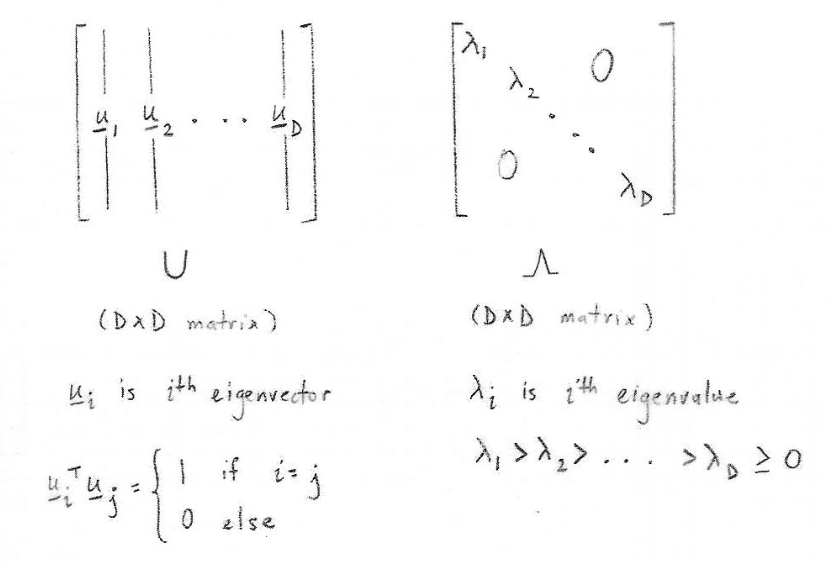
\includegraphics[scale=0.5]{Eigendecomposition.png}
\end{center}

Note that $\mathbf{u}_1,\ldots\mathbf{u}_D$ form an orthonormal basis for
$\mathbb{R}^D$. In other words, any point in $\mathbb{R}^D$ can be expressed as
a linear combination of the $\mathbf{u}_1,\ldots\mathbf{u}_D$.

\subsection{Principal Component directions}
\begin{itemize}
  \item The first PC direction, $\mathbf{u}_1$, captures the greatest data
  variance.

  \item The second PC direction ($\mathbf{u}_2$) captures the second
  greatest data variance and is orthogonal to $\mathbf{u}_1$.

  \item And so on...
\end{itemize}

\begin{minipage}{0.5 \textwidth}
  Another way of saying that the PC directions are a basis is that \underline{they
  define a new set of coordinate axes}. This means that a data point $\xb_n \in
  \mathbb{R}^2 = \begin{bmatrix} x_n^{(1)} \\ x_n^{(2)} \end{bmatrix}$ can
  equivalently be described in the new coordinate system as $\zb_n =
  \begin{bmatrix} z_n^{(1)} \\ z_n^{(2)} \end{bmatrix}$.
\end{minipage}\hfill
\begin{minipage}{0.45 \textwidth}
  \begin{center}
    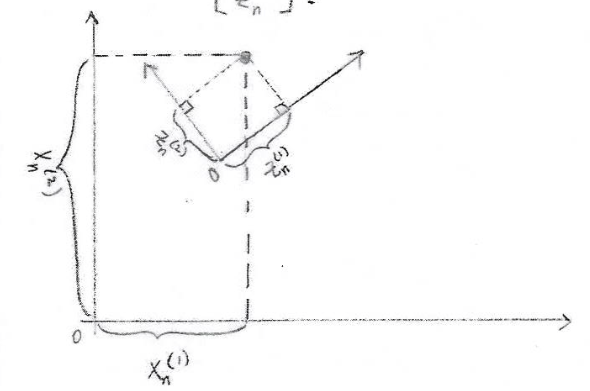
\includegraphics[width=\textwidth]{PCADimensions.png}
  \end{center}
\end{minipage}

\begin{minipage}{0.7 \textwidth}
  \textit{How do we relate $\xb_n$ and $\zb_n$?}

  In general, if we have two vectors,
  $\mathbf{v}$ and $\Wb$, the projection of $\mathbf{v}$ onto
  $\Wb$ is
  \begin{equation}
    \lVert \mathbf{v} \rVert \cos \theta =
    \frac{\lVert \mathbf{v} \rVert \lVert \Wb \rVert \cos \theta}
    {\lVert \Wb \rVert}
    = \frac{\mathbf{v}\tran\Wb}{\lVert \Wb \rVert}
    \label{eqn:projection}
  \end{equation}
\end{minipage}\hfill
\begin{minipage}{0.25 \textwidth}
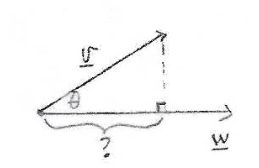
\includegraphics[width=\textwidth]{Projection.png}
\end{minipage}

\subsection{Projecting into PCA dimensions}
In order to project from our high-dimensional data space
($\xb \in \mathbb{R}^D$) into our lower dimensional PC space
($\zb \in \mathbb{R}^M$)
\begin{framed}
  \begin{equation}
    z^{(i)} = (\xb - \ub)\tran \mathbf{u}_i, \, i = 1, \ldots, M
  \end{equation}
\end{framed}
The coordinates in PC space are also called \textbf{``PC scores''}. Intuitively,
this means that we center the high-dimensional data, and then project onto
the axes defined by the $\mathbf{u}_i$'s (remember that
$\Vert \mathbf{u}_i \rVert = 1$, so the denominator in \eqref{eqn:projection} is
1). This is illustrated for $D=2$ and $M=1$ below.
\begin{center}
  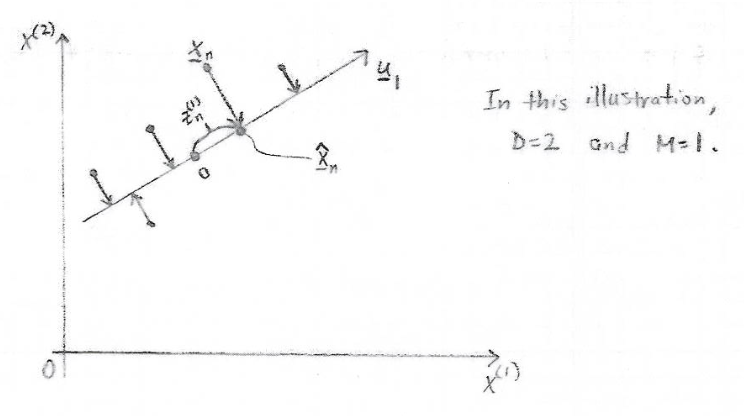
\includegraphics[scale=0.5]{ProjectionExample.png}
\end{center}
If we define $\mathbf{U}_M$ as the first $M$ columns of the eigenvector matrix
$\mathbf{U}$ above (i.e., $\mathbf{U}_M = [\mathbf{u}_1 \mathbf{u}_2, \ldots,
\mathbf{u}_M ]$), then we can write the projection in vector form
\begin{equation*}
  \zb = {\mathbf{U}_M}\tran (\xb - \ub).
\end{equation*}


\subsection{``Back-projecting'' reduced dimensional data}
In low-dimensional coordinates, the projection of $\xb_n$ is $\zb_n$. What does
$\zb_n$ look like back in the original coordinate system?
\begin{framed}
  \begin{equation}
    \hat{\xb}_n = \sum_{i=1}^M z_n^{(i)} \mathbf{u}_i + \ub =
    \mathbf{U}_M \zb
  \end{equation}
\end{framed}
Because we've initially projected $\xb$ into a low-dimensional space, we call
estimating $\hat{\xb}_n$ ``projecting back into the high-dimensional space.''

\textit{Thought question:}
\begin{equation*}
  \text{What is} \; \sum_{i=1}^D z_n^{(i)} \mathbf{u}_i + \ub?
\end{equation*}
\textit{Answer:} It's just $\xb_n$!

\subsection{How to choose M?}
So when we're doing PCA, how do we choose how many eigenvectors to include
in our lower dimensional representation; what value of $M < D$ should we pick?

Eigendecompositions always sort the eigenvectors by eigenvalue. So, if we plot
the eigenvalue ``spectrum'' of $\mathbf{S}$, we can look for an ``elbow''.
\begin{center}
  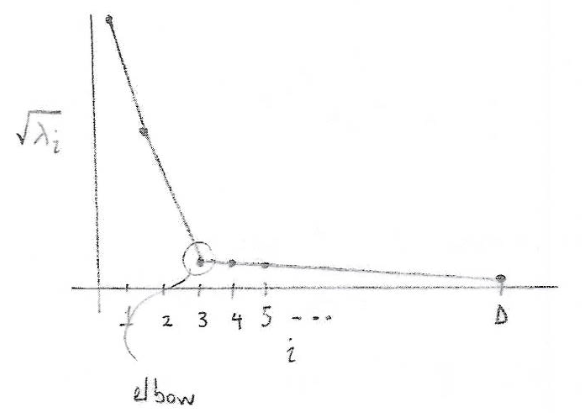
\includegraphics[scale=0.5]{Eigenspectrum.png}
\end{center}
The typical instruction is to choose $M$ to be the number of eigenvalues above
the elbow. So in the example above, one would choose $M=2$. In many cases, one
does not actually see a clear-cut elbow. This is one of the motivations of a
probabilistic model-based approach to dimensionaity reduction, such as
probabilistic PCA (P-PCA) (which we'll introduce in the next section), where
one can use cross-validated likelihoods to determine $M$.

With PCA, it can be shown that the fraction (percentage) of variance in the
data which is explained by the first $M$ eigenvectors (principal components)
can be found from the eigenvalues
\begin{equation*}
  \text{Fraction of variance explained by $M < D$ eigenvectors } =
  \frac{\sum_{i=1}^M \lambda_i}{\sum_{i=1}^D \lambda_i}.
\end{equation*}


\begin{propertybox}
  \textbf{Note:} We described PCA in terms of \underline{maximizing the
  variance of the projected data}. Equivalently, we could have formulated PCA
  in terms of \underline{minimizing the projection error}.
\end{propertybox}

\begin{framed}
\subsection{Summary of PCA}
\begin{description}[%
  before={\setcounter{descriptcount}{0}},%
  ,font=\bfseries\stepcounter{descriptcount}\thedescriptcount.~]

  \item{\underline{Data set:}} $\xb_b \in \mathbb{R}^D, n = 1, \ldots, N$

  \item{\underline{Find the sample covariance, $\mathbf{S}$, and
    mean, $\ub$:}}
    \begin{align*}
      \mathbf{S} &= \frac{1}{N} \sum_{n=1}^N (\xb-\ub) (\xb-\ub)\tran \\
      \ub &= \frac{1}{N} \sum_{n=1}^N \xb
    \end{align*}

  \item{\underline{Diagonalize $\mathbf{S}$}}
    \begin{equation*}
      \mathbf{S} = \mathbf{U} \symbf{\Lambda} \mathbf{U}\tran
    \end{equation*}
    where $\symbf{\Lambda}$ is a diagonal matrix with ordered eigenvalues on the
    diagonal, and $\mathbf{U}$ contains the eigenvectors
    \begin{equation*}
      \begin{bmatrix}
        \vline height 1.5 em & \vline &   & \vline \\
        \mathbf{u}_1 & \mathbf{u}_2 & \ldots & \mathbf{u}_D \\
        \vline  height 1.5 em & \vline &   & \vline
      \end{bmatrix}
    \end{equation*}
  \item{\underline{Choose $M$:}}
    Choose the number of reduced dimensions $M < D$. Define
    \begin{equation*}
      \mathbf{U}_M =
      \begin{bmatrix}
        \vline height 1.5 em & \vline &   & \vline \\
        \mathbf{u}_1 & \mathbf{u}_2 & \ldots & \mathbf{u}_M \\
        \vline  height 1.5 em & \vline &   & \vline
      \end{bmatrix}
    \end{equation*}

  \item{\underline{PC directions}} are the columns of $\mathbf{U}_M$.

  \item{\underline{PC scores:}}
    \begin{equation*}
      \zb_n = {\mathbf{U}_M} \tran (\xb_n - ub), \quad \zb_n \in \mathbb{R}^M
    \end{equation*}
    The ``PC score'' for a data point $\xb_n$ is its low-dimensional projection,
    $\zb_n$.

  \item{\underline{Back-projection:}}
    The low-dimensional point can be projected back into the data space:
    \begin{align*}
      \hat{\xb}_n &= \mathbf{U}_M \zb_n + \ub \\
        &= \mathbf{U}_M {\mathbf{U}_M}\tran (\xb_n - \ub) + \ub
    \end{align*}
\end{description}
\end{framed}

\begin{propertybox}
  \textbf{Note:} The PC directions are only unique up to a sign difference. In
  other words, the $i^{\text{th}}$ PC direction can be $\mathbf{u}_i$ or
  $-\mathbf{u}_i$. This will determine the sign of the $i^{\text{th}}$ PC
  score (i.e., $z^{(i)}$).
\end{propertybox}

\section{Probabilistic PCA}
In the last section we described traditional principal components analysis as
formulated as a linear projection into an orthogonal lower dimensional space
which maximizes variance (or minimizes projection error). Next we will describe
a latent variable model for dimensionality reduction. The maximum likelihood
solution for this P-PCA model will end up yielding a nearly identical solution
as PCA but with some key advantages.

\subsection{Advantages of P-PCA over conventional PCA}
By virtue of being a probabilistic model, Probabilistic PCA has advantages over
traditional PCA.
\begin{itemize}
  \item P-PCA assigns probabilities to data, so we can compare different models --
  particularly with different values of the reduced number of dimensions, $M$ --
  using cross-validated data likelihoods.

  \item P-PCA has an explicit noise model, so it can more effectively remove
  ``noise'' (i.e., variability not explained by variation in the low-dimensional
  space).

  \item If the data dimensionality, $D$, is large, calculation of the
  eigenvectors of the covariance matrix can be an $O(D^3)$ operation. The
  EM algorithm solution for P-PCA gives a nice (and more simple) way to
  compute just the first $M$ eigenvectors.

  \item Because it is a probabilistic model, with P-PCA one can learn the
  low-dimensional space when there is missing data. There is no principled way
  to modify the PCA algorithm in this condition.
  \begin{center}
    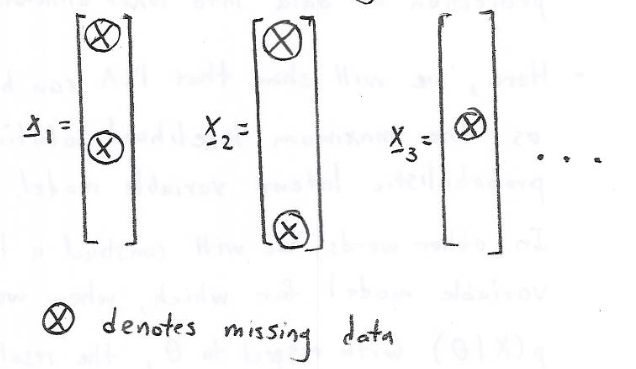
\includegraphics[scale=0.5]{MissingData.png}
  \end{center}

  \item Because P-PCA is a probabilistic model, we can easily propose extensions
  like mixtures of P-PCA models (which would be analogous to mixtures of
  Gaussians).

  \item Like all probabilistic latent variable models, P-PCA is generative,
  so one can generate synthetic samples to examine.
\end{itemize}

\subsection{Generative model for P-PCA}
\begin{flalign*}
  \xb \in \mathbb{R}^D & \text{is high dimensional observed data} \\
  \zb \in \mathbb{R}^M & \text{is a lower dimensional latent variable}
\end{flalign*}
\begin{equation}
\begin{aligned}
  \Pr (\zb) &= \mathcal{N}(\mathbf{0}, \mathbf{I}) && \text{``state model''} \\
  \Pr (\xb \mid \zb) &=
\mathcal{N}(\underbrace{\Wb}_{\mathllap{\text{$D \times M$ matrix}}}
  \zb + \ub, \underbrace{\sigma^2}_{\mathrlap{\text{``observation noise''}}}
      \mathbf{I}) \qquad \qquad && \text{``observation model''}
\end{aligned}
\end{equation}
\begin{propertybox}
\textit{Looking ahead:} If we fit this model to data $\xb_1, \ldots, \xb_N$ --
that is if we find the model parameters $\theta = \{\Wb, \ub, \sigma^2\}$
which maximize the data likelihood -- the columns of $\Wb$ will span the
same space as the PCA principal components (i.e., the columns of $\mathbf{U}_M$).
In the limit of $\sigma^2 \rightarrow 0$, the low-dimensional projections of
P-PCA approach those of PCA.
\end{propertybox}

Here is a picture of the P-PCA model where $M=1$ and $D=2$:
\begin{center}
  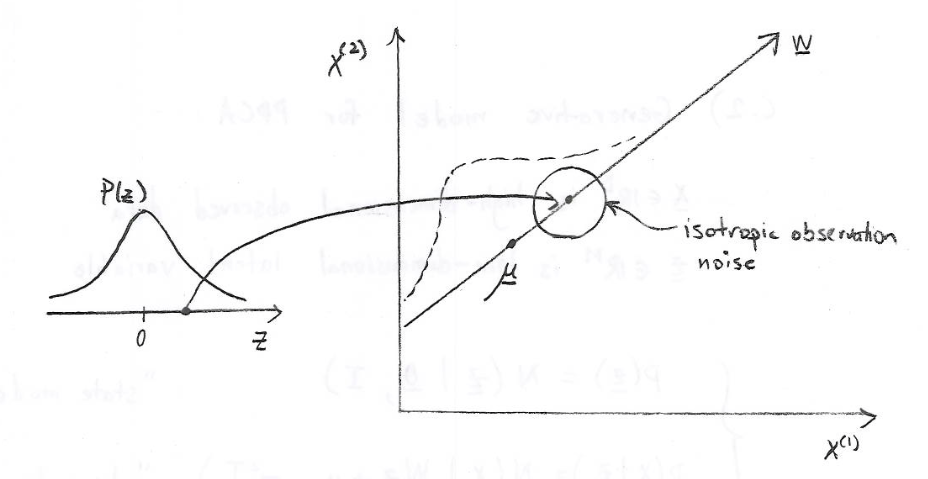
\includegraphics[scale=0.5]{PPCASchema.png}
\end{center}

\subsection{P-PCA is a linear Gaussian model}

Since the latent variable model and the observation model have Gaussian
variability and the observations ($\xb$) are \underline{linearly related} to the
latent variables ($\zb$) P-PCA falls into a very convenient model category --
the ``linear Gaussian  model''. For these models all the marginal, conditional,
and joint distributions are Gaussian!
\begin{equation*}
  \begin{aligned}
    \Pr(\xb), \Pr(\zb): & \quad && \text{Marginal distributions} \\
    \Pr(\xb \mid \zb), \Pr(\zb \mid \xb): & \quad && \text{Conditional distributions} \\
    \Pr(\xb, \zb):& \quad && \text{Joint distribution}
  \end{aligned}
\end{equation*}
Since these distributions are all Gaussian, we can specify them completely by
their means and covariances. Our model specifies $\Pr(\zb)$ and $\Pr(\xb \mid
\zb)$, so lets find the parameters of the other distributions.

\subsubsection{$\Pr(\xb,\zb)$}
\begin{equation*}
  \begin{bmatrix}\zb \\ \xb\end{bmatrix} \sim
    \mathcal{N}\left( \begin{bmatrix}\E(\zb) \\ \E(\xb)\end{bmatrix},
      \begin{bmatrix}\Cov(\zb) & \E(\zb \, \xb\tran) - \E(\zb)\E(\xb)\tran \\
                     \E(\xb \, \zb\tran) - \E(\xb)\E(\zb)\tran & \Cov(\xb)\end{bmatrix}
    \right)
\end{equation*}

\begin{equation*}
  \E(\zb) = 0 \tag*{From model specification}
\end{equation*}

An equivalent way of describing our observations is
\begin{equation}
  \xb = \Wb\, \zb + \ub + \symbf{\epsilon}, \text{where }
    \symbf{\epsilon} \sim \mathcal{N} (\mathbf{0}, \sigma^2 \mathbf{I})
  \label{eqn:lgModel}
\end{equation}
Note that since we have originally specified this as the conditional
distribution of $\xb$ given $\zb$, this implies that $\symbf{\epsilon}$ is
independent of $\zb$. Taking the expectation over both $\zb$ and
$\symbf{\epsilon}$ (since we're interested in the \textit{joint} distribution),
we find
\begin{align*}
  \E(\mathbf{x}) &= \E(\Wb\,\zb + \ub + \symbf{\epsilon}) \\
  &= \Wb\; \cancelto{0}{\E(\zb)} + \ub + \cancelto{0}{\E(\symbf{\epsilon}} \\
  &=\ub
\end{align*}

\begin{equation*}
  \Cov(\zb) = \mathbf{I} \tag*{From model specification}
\end{equation*}

\begin{align*}
  \Cov(\xb) &= \E(\xb\, \xb\tran) - \E(\xb) \E(\xb)\tran \\
  &= \E\left(
      (\Wb\,\zb + \ub + \symbf{\epsilon})
      (\Wb\,\zb + \ub + \symbf{\epsilon})\tran \right) -
      \ub \ub \tran \\
  &= \E(\Wb\, \zb \zb\tran \Wb\tran +
        \cancelto{0}{\Wb\, \zb \ub \tran} +
        \Wb\, \zb \symbf{\epsilon}\tran +
        \cancelto{0}{\ub \zb\tran \Wb\tran} +
        \ub \ub \tran +
        \cancelto{0}{\ub \symbf{\epsilon}\tran} +
        \symbf{\epsilon} \zb\tran \Wb\tran +
        \cancelto{0}{\symbf{\epsilon} \ub \tran} +
        \symbf{\epsilon} \symbf{\epsilon}\tran) - \ub \ub \tran\\
  &\quad \text{where we have cancelled all products of constants and zero mean variables} \\
  &= \E(\Wb\, \zb \zb\tran \Wb\tran +
        \cancelto{0}{\Wb\, \zb \symbf{\epsilon}\tran} +
        \ub \ub \tran +
        \cancelto{0}{\symbf{\epsilon} \zb\tran \Wb\tran} +
        \symbf{\epsilon} \symbf{\epsilon}\tran) - \ub \ub\tran
        \tag*{Because $\symbf{\epsilon}$ and $\zb$ are independent.}\\
  &= \Wb \E(\zb \zb\tran) \Wb\tran +
        \E(\symbf{\epsilon} \symbf{\epsilon}\tran) \\
  &= \Wb\,\Wb\tran + \sigma^2 \mathbf{I} \tag*{From the definitions}
\end{align*}

\begin{align*}
  \E(\xb \, \zb\tran) - \E(\xb)\E(\zb)\tran &=
  \E\left((\Wb\,\zb + \ub + \symbf{\epsilon}) \zb\tran\right) - \mathbf{0} \\
  &= \Wb\E(\zb \zb\tran) +
  \ub\cancelto{0}{\E(\zb\tran)} +
  \cancelto{0}{\E(\symbf{\epsilon}\zb\tran)} \\
  &= \Wb
\end{align*}

So, plugging in, we have the joint distribution
\begin{equation}
  \begin{bmatrix}\zb \\ \xb\end{bmatrix} \sim
    \mathcal{N}\left( \begin{bmatrix} \mathbf{0} \\ \ub\end{bmatrix},
      \begin{bmatrix}\mathbf{I} & \Wb\tran \\
                     \Wb &
            \Wb\,\Wb\tran + \sigma^2\mathbf{I}\end{bmatrix}
    \right)
  \label{eqn:joint}
\end{equation}

\subsubsection{$\Pr(\xb)$}
We can read the marginal distribution directly from \eqref{eqn:joint}.
\begin{equation}
  \Pr(\xb) \sim \mathcal{N}(\ub, \Wb\,
      \Wb\tran + \sigma^2\mathbf{I})
  \label{eqn:marginalX}
\end{equation}

\subsubsection{$\Pr(\zb \mid \xb)$}
In order to find the other marginal distribution, we could write down the
equations and use Bayes rule and a bunch of linear algebra to simplify.
Easier is to make use of a useful factoid (see \textit{PRML} Section 2.3.1):
\begin{framed}
  \underline{Conditioning for multivariate Gaussian random variables}

  If $\xb = \begin{bmatrix}\xb_a \\ \xb_b\end{bmatrix} \sim
  \mathcal{N}\left( \begin{bmatrix} \ub_a \\ \ub_b \end{bmatrix},
    \begin{bmatrix}\Sb_{aa} & \Sb_{ab} \\
                   \Sb_{ba} & \Sb_{bb} \end{bmatrix}
  \right)$ then $\Pr(\xb_a \mid \xb_b)$ is Gaussian with mean
  \begin{equation*}
    \E(\xb_a \mid \xb_b) = \ub_a + \Sb_{ab} \Sb_{bb}^{-1} (\xb_b-\ub_b)
  \end{equation*}
  and covariance
  \begin{equation*}
    \Cov(\xb_a \mid \xb_b) = \Sb_{aa} - \Sb_{ab} \Sb_{bb}^{-1} \Sb_{ba}
  \end{equation*}

  Let's try to make intuitive sense of these equations. Basically, once we
  we observe $\xb_b$, we should modify our estimate of $\xb_a$ (the
  $\Sb_{ab}$ term), but weighted by how noisy $\xb_b$ is (the
  $\Sb_{ab}^{-1}$ term). And once we make that new estimate, the covariance
  decreases -- we believe that we know a little more about $\xb_a$ than we did
  before. The amount of that decrease doesn't depend on the actual measurement
  of $\xb_b$, just on it's covariance and the transformation from one space to
  the other (the $\Sb_{ab} \Sb_{bb}^{-1} \Sb_{ba}$ term).
\end{framed}

Plugging in from \eqref{eqn:joint}, we have
\begin{align*}
  \E(\zb \mid \xb) &= \mathbf{0} + \Wb\tran \mathbf{C}^{-1}(\xb-\ub) \\
  \Cov(\zb \mid \xb) &= \mathbf{I} - \Wb\tran \mathbf{C}^{-1} \Wb,
\end{align*}
where $C = \Wb \, \Wb\tran + \sigma^2 \mathbf{I}$.

Thus,
\begin{equation}
  \zb \mid \xb \sim \mathcal{N} (\Wb\tran \mathbf{C}^{-1} (\xb-\ub),
      \mathbf{I} - \Wb\tran \mathbf{C}^{-1}\Wb)
  \label{eqn:obsConditional}
\end{equation}

\subsection{EM Algorithm for P-PCA}
\begin{center}
  \textbf{Goal:} Maximize $\log \Pr(\{\xb\} \mid \theta)$ where
    $\theta = \{\Wb, \ub, \sigma^2$\}.
\end{center}
The EM algorithm will find an exact solution for the mean, $\ub$,
and iteratively optimize values of $\Wb$ and $\sigma^2$ such that the
sample covariance is
\begin{equation*}
  \mathbf{S} \approx \Wb\,\Wb\tran + \sigma^2 \mathbf{I}.
\end{equation*}
This makes sense if we look back at \eqref{eqn:marginalX}.

The maximum likelihood solution for the mean is just the sample mean, which
we're not going to show.

\subsubsection*{E-Step:}
Find $\Pr(\zb_n \mid \xb_n)$ for each data point using \eqref{eqn:obsConditional}.

\subsubsection*{M-Step:}
\begin{align*}
  \log \Pr({\xb}_N, {\zb}_N) &= \sum_{n=1}^N \log\Pr(\xb_n, \zb_n) \\
  &= \sum_{n=1}^N (\log\Pr(\xb_n \mid \zb_n) + \log\Pr(\zb_n)) \\
  &= \sum_{n=1}^N \Bigl(
    -\frac{D}{2}\log(2\pi) -\frac{1}{2}\logdet{\sigma^2 \mathbf{I}}
    -\frac{1}{2}(\xb_n - \Wb\, \zb_n - \ub)\tran (\sigma^2 \mathbf{I})^{-1}
            (\xb_n - \Wb\, \zb_n - \ub) \\
  &\quad\qquad -\frac{M}{2}\log(2\pi) -\cancelto{0}{\frac{M}{2}\logdet{\mathbf{I}}}
    -\frac{1}{2}\zb\tran \zb \Bigr)
\end{align*}
\begin{align*}
  Q &= \E_{\zb\mid\xb} (\log \Pr({\xb}_N, {\zb}_N)) \\
  &= \sum_{n=1}^N \Bigl(
    -\frac{D}{2}\log(2\pi \sigma^2)
    -\frac{1}{2 \sigma^2} \E_{\zb\mid\xb}\Bigl((\xb_n - \ub - \Wb\, \zb_n )\tran
          (\xb_n - \ub - \Wb\, \zb_n)\Bigr) \\
  &\quad \qquad -\frac{M}{2}\log(2\pi) -\frac{1}{2}\E_{\zb\mid\xb}(\zb\tran \zb) \Bigr) \\
  &= \sum_{n=1}^N \Bigl(-\frac{D}{2}\log(2\pi \sigma^2)
    -\frac{1}{2 \sigma^2} \Bigl((\xb_n - \ub)\tran(\xb_n - \ub))
    -\E_{\zb\mid\xb}(\zb_n\tran \Wb\tran (\xb_n - \ub)) \\
  &\quad \qquad  -\E_{\zb\mid\xb}((\xb_n - \ub)\tran \Wb\, \zb_n)
    +\E_{\zb\mid\xb}(\zb_n\tran \Wb\tran \Wb\, \zb_n)\Bigr) \\
  &\quad \qquad -\frac{M}{2}\log(2\pi) -\frac{1}{2}\E_{\zb\mid\xb}(\zb\tran \zb) \Bigr) \\
  &= \sum_{n=1}^N \Bigl(-\frac{D}{2}\log(2\pi \sigma^2)
    -\frac{1}{2 \sigma^2} \Bigl((\xb_n - \ub)\tran(\xb_n - \ub))
    -\E_{\zb\mid\xb}(\zb_n)\tran \Wb\tran (\xb_n - \ub) \\
  &\quad \qquad  -(\xb_n - \ub)\tran \Wb\, \E_{\zb\mid\xb}(\zb_n)
    +\Tr(\Wb\tran \Wb\E_{\zb\mid\xb}(\zb_n \zb_n\tran))\Bigr) \\
  &\quad \qquad -\frac{M}{2}\log(2\pi) -\frac{1}{2}\E_{\zb\mid\xb}(\zb_n\tran \zb_n) \Bigr) \\
\end{align*}
\begin{gather*}
  \frac{\partial Q}{\partial \Wb} =
  \sum_{n=1}^N -\frac{1}{2 \sigma^2}\Bigl(
    -(\xb_n - \ub) \E_{\zb\mid\xb}(\zb_n) \tran
    -(\xb_n - \ub) \E_{\zb\mid\xb}(\zb_n) \tran
    + 2 \Wb \E_{\zb\mid\xb}(\zb_n\, \zb_n\tran) \Bigr) = 0 \\
  \implies \Wb \Bigl(\sum_{n=1}^N \E_{\zb\mid\xb}(\zb_n\, \zb_n\tran) \Bigr) =
  \sum_{n=1}^N (\xb_n - \ub) \E_{\zb\mid\xb}(\zb_n) \tran
\end{gather*}
\begin{framed}
  \begin{equation}
    \Wb_{new} = \Bigl(\sum_{n=1}^N (\xb_n - \ub) \E_{\zb\mid\xb}(\zb_n) \tran \Bigr)
    \Bigl(\sum_{n=1}^N \E_{\zb\mid\xb}(\zb_n\, \zb_n\tran) \Bigr)^{-1}
  \end{equation}
\end{framed}
\begin{gather*}
  \frac{\partial Q}{\partial \sigma^2} =
  \sum_{n=1}^N -\frac{D}{2}\frac{1}{\sigma^2}
    + \frac{1}{2} \frac{1}{(\sigma^2)^2}
  \Bigl( \; \cdot \; \Bigr) = 0 \\
  -N D + \frac{1}{\sigma^2} \sum_{n=1}^N \Bigl( \; \cdot \; \Bigr) = 0 \\
  \implies  \sigma^2 = \frac{1}{N D} \sum_{n=1}^N \Bigl( \; \cdot \; \Bigr) \\
  \implies \sigma^2 = \frac{1}{N D} \sum_{n=1}^N
    \Bigl((\xb_n - \ub)\tran(\xb_n - \ub))
    -\E_{\zb\mid\xb}(\zb_n)\tran \Wb\tran (\xb_n - \ub) \\
  \quad \qquad  -(\xb_n - \ub)\tran \Wb\, \E_{\zb\mid\xb}(\zb_n)
    +\Tr(\Wb\tran \Wb\E_{\zb\mid\xb}(\zb_n \zb_n\tran))\Bigr)
\end{gather*}
This is a complicated expression, but looking back, we remember that
\begin{equation*}
  \sum_{n=1}^N (\xb_n - \ub) \E_{\zb\mid\xb}(\zb_n) \tran =
  \Wb_{new} \Bigl(\sum_{n=1}^N \E_{\zb\mid\xb}(\zb_n\, \zb_n\tran) \Bigr),
\end{equation*}
and note that all the individual expressions are scalars and thus can be wrapped
in a trace operation.

Plugging this in, we have
\begin{align*}
   \sigma^2 &= \frac{1}{N D} \Biggl(
    \Tr\Bigl(\sum_{n=1}^N (\xb_n - \ub)\tran(\xb_n - \ub)\Bigr)
    -\Tr\Bigl(\sum_{n=1}^N \E_{\zb\mid\xb}(\zb_n)\tran \Wb\tran (\xb_n - \ub)\Bigr) \\
    & \quad
    -\Tr\Bigl(\sum_{n=1}^N (\xb_n - \ub)\tran \Wb\, \E_{\zb\mid\xb}(\zb_n)\Bigr)
    +\Tr\Bigl(\sum_{n=1}^N \Wb\tran \Wb\E_{\zb\mid\xb}(\zb_n \zb_n\tran)\Bigr)
  \Biggr) \\
  &= \frac{1}{N D} \Biggl(
    \Tr\Bigl(\sum_{n=1}^N (\xb_n - \ub)\tran (\xb_n - \ub)\Bigr)
    -\Tr\Bigl(\Wb\tran \overbrace{\sum_{n=1}^N (\xb_n - \ub)\E_{\zb\mid\xb}(\zb_n)\tran}\Bigr) \\
    & \quad
    -\Tr\Bigl(\Wb \sum_{n=1}^N \E_{\zb\mid\xb}(\zb_n)(\xb_n - \ub)\tran\Bigr)
    +\Tr\Bigl(\sum_{n=1}^N \Wb\tran \Wb\E_{\zb\mid\xb}(\zb_n \zb_n\tran)\Bigr)
  \Biggr) \\
  &= \frac{1}{N D} \Biggl(
    \Tr\Bigl(\sum_{n=1}^N (\xb_n - \ub)\tran (\xb_n - \ub)\Bigr)
    -\cancel{\Tr\Bigl(\Wb\tran \overbrace{\Wb_{new} \Bigl(\sum_{n=1}^N \E_{\zb\mid\xb}(\zb_n\, \zb_n\tran) \Bigr)} \Bigr)} \\
    & \quad
    -\Tr\Bigl(\Wb\sum_{n=1}^N \E_{\zb\mid\xb}(\zb_n)(\xb_n - \ub)\tran\Bigr)
    +\cancel{\Tr\Bigl(\sum_{n=1}^N \Wb\tran \Wb\E_{\zb\mid\xb}(\zb_n \zb_n\tran)\Bigr)}
  \Biggr) \\
\end{align*}
Making sure that all of our traces are over the same dimension of matrices we
can combine to get our final result:
\begin{framed}
  \begin{equation}
    \sigma^2_{new} = \frac{1}{N D} \Tr \Biggl(
      \sum_{n=1}^N (\xb_n - \ub) (\xb_n - \ub) \tran
      - \Wb_{new}\sum_{n=1}^N \E_{\zb\mid\xb}(\zb_n)(\xb_n - \ub)\tran
    \Biggr)
  \end{equation}
\end{framed}

\begin{propertybox}
  \textbf{Implementation Aside:} A common error in implementing the EM algorithm
  is for students to confuse $\E_{\zb\mid\xb}(\zb_n\, \zb_n\tran)$ for the
  covariance in \eqref{eqn:obsConditional}. Rather, it is the expected outer
  product,

  $\E_{\zb\mid\xb}(\zb_n\, \zb_n\tran) = \Cov(\zb_n \mid \xb_n) +
  \E(\zb_n\mid\xb_n) \E(\zb_n\mid\xb_n)\tran$
\end{propertybox}

\subsection{Relating P-PCA to PCA}
\subsubsection*{PC Directions}
The columns of $\Wb$ for P-PCA span \underline{the same space} as that spanned
by the columns of $\mathbf{U}_M$ from PCA. The difference between them is that
the columns of $\mathbf{U}_M$ are orthonormal and ordered based on the amount
of variance explained. Neither of these aspects will in general be true for
$\Wb$.

However, with some linear algebra one can obtain $\mathbf{U}_M$ from $\Wb$.
Specifically, we can calculate the singular value decomposition (SVD) of $\Wb$.
The SVD is a generalization of the eigendecomposition for non-square matrices.
\begin{center}
  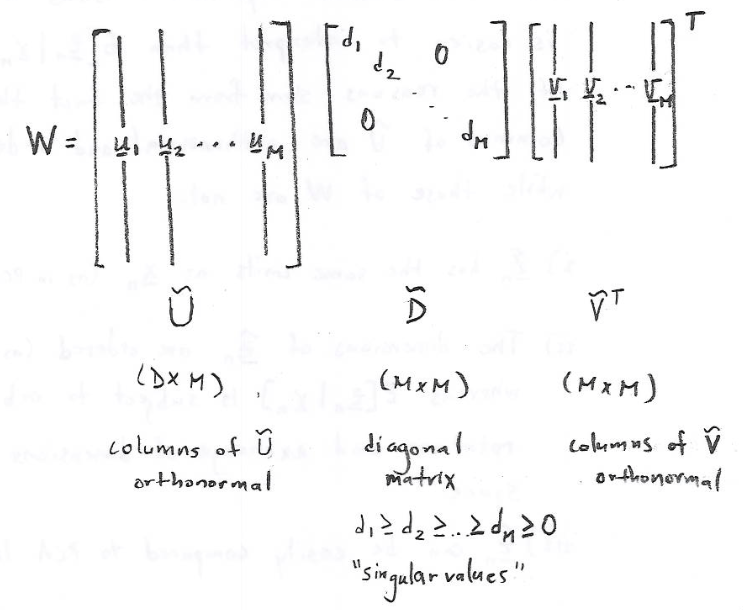
\includegraphics[scale=0.5]{SVD.png}
\end{center}
The matrix $\tilde{\mathbf{U}}$ calculated from $\Wb$ in P-PCA will be identical
(in the limit of EM convergence) to $\mathbf{U}_M$ for PCA.

\subsubsection*{Low-dimensional projections}
In P-PCA, the low-dimensional projection corresponding to $\Wb$ is $\E(\zb_n
\mid \xb_n) = \Wb\tran \mathbf{C}^{-1}(\xb_n - \ub)$ from
\eqref{eqn:obsConditional}. The same point can be back-projected to the
original state by
\begin{align*}
  \hat{\xb}_n &= \Wb \E(\zb_n \mid \xb_n) + \ub \\
  &= \tilde{\mathbf{U}} \underbrace{\tilde{\mathbf{D}} \tilde{\mathbf{V}}\tran
    \E(\zb_n \mid \xb_n)}_{\mathclap{\text{\normalsize call this $\tilde{\zb}_n$}}} + \ub
\end{align*}
There are several important reasons why $\tilde{\zb}_n$ is easier to interpret
than $\E(\zb_n \mid \xb_n)$. All of the reasons stem from the fact that the
columns of $\tilde{\mathbf{U}}$ are orthonormal and ordered while those of $\Wb$
are not.
\begin{enumerate}
  \item $\tilde{\zb}_n$ has the same units as $\xb_n$ (as in PCA)
  \item The dimensions of $\tilde{\zb}_n$ are ordered (as in PCA), whereas
  $\E(\zb_n \mid \xb_n)$ can be arbitrarily rotated and scaled in the latent
  space.
  \item $\tilde{\zb}_n$ can be easily compared to the low-dimensional PCA
  projection.
\end{enumerate}

How does the low-dimensional projection for P-PCA ($\tilde{\zb}_n$) compare
with that of PCA ($\mathbf{U}_M (\xb_n - \ub)$)? Without proof,
\begin{equation}
  \tilde{\zb}_n =
  \begin{bmatrix}
    \frac{\lambda_1 - \sigma^2}{\lambda_1} & \multicolumn{2}{c}{0} \\
     & \ddots &  \\
    \multicolumn{2}{c}{0} & \frac{\lambda_M - \sigma^2}{\lambda_M} \\
  \end{bmatrix}
  \mathbf{U}_M (\xb_n - \ub)
\end{equation}
Unpacking, this means that the low-dimensional projection for P-PCA shrinks
the PCA low-dimensional projection to the origin in $\zb$-space, because $0
\leq \frac{\lambda_i - \sigma^2}{\lambda_i} \leq 1$. Furthermore, as
$\sigma^2 \rightarrow 0$, the P-PCA projections converge to the PCA projections.

\subsubsection*{Intuition for P-PCA vs PCA}
Each of these models is trying to explain the variability of $\xb$ away from
its mean $\ub$. P-PCA can explain this variability as a combination of variation
in low-dimensional space -- the latent variable $\zb$ -- and observation noise,
$\symbf{\epsilon} \sim \mathcal{N}(\mathbf{0},\sigma^2 \mathbf{I})$. But how
much of each?

As $\sigma^2$ increases (more observation noise), the proportion of the
variability attributed to observation noise increases, and the proportion
attributed to the latent space decreases, shrinking $\zb$ to its mean (which
is zero, corresponding to $\mu$ in the data space). PCA is the opposite limit;
as $\sigma^2$ decreases to zero, there  is no observation noise, and all
variability of $\xb$ from $\ub$ must be explained by the latent variable space.
Thus, \textit{P-PCA is more effective at denoising data than PCA}.

\subsection{Redux - Advantages of P-PCA over PCA}
\begin{itemize}
  \item The dimensionality, $M$, of the latent space for P-PCA can be selected
  using cross-validated likelihoods, where $\Pr(\{\xb\}_N)$ is given in
  \eqref{eqn:marginalX}.

  \item P-PCA defines a constrained Gaussian in \eqref{eqn:marginalX}, with
  $\Cov(\xb) = \Wb\,\Wb\tran + \sigma^2 \mathbf{I}$, which is a useful
  compromise between a Gaussian with diagonal covariance (too constraining in
  many situations) and a Gaussian with a full covariance matrix
  (underconstrained in the scenarios where we would want to employ
  dimensionality reduction).
\end{itemize}

\section{Factor Analysis (FA)}
\subsection{Motivation}
P-PCA assumes that the observation noise is ``isotropic'' -- the same in all
observation dimensions. This makes sense if each dimension is a similar
measurement, but if they are different (i.e., height and weight), we would
like each dimension of $\xb$ to have a different level of observation noise.

The \underline{only} difference between FA and P-PCA is that instead of
modeling the covariance of the observation noise as $\sigma^2 \mathbf{I}$ (in
\eqref{eqn:lgModel}), the observation noise covariance is a diagonal matrix
$\symbf{\Psi}$. So, for FA
\begin{equation}
  \xb \sim \mathcal{N}(\mu, \Wb\,\Wb\tran + \symbf{\Psi}),
  \label{eqn:faCov}
\end{equation}
where the similarity to \eqref{eqn:marginalX} is clear.

We can define an EM algorithm that is nearly identical to P-PCA. When solving for
the M-step, after replacing all the instances of $\sigma^2 \mathbf{I}$ with
$\symbf{\Psi}$, the update for $\Wb$ is unchanged and the update for the
covariance becomes
\begin{framed}
  \begin{equation}
    \symbf{\Psi}_{new} = \frac{1}{N} \diag \Biggl(
      \sum_{n=1}^N (\xb_n - \ub) (\xb_n - \ub) \tran
      - \Wb_{new}\sum_{n=1}^N \E_{\zb\mid\xb}(\zb_n)(\xb_n - \ub)\tran
    \Biggr)
  \end{equation}
\end{framed}
where the $\diag()$ operator zeros the off-diagonal elements. For the E-step,
everything is the same except the marginal covariance of $\xb$ ($C$ in
\eqref{eqn:obsConditional}) is given by \eqref{eqn:faCov}.

\subsubsection{Comparing FA and P-PCA}
Because of the non-isotropic observation noise, FA will identify different
latent dimensions within the data space than P-PCA/PCA. As with P-PCA, we will
need to orthonormalize the columns of $\Wb$ for interpretability.
\begin{itemize}
  \item PCA/P-PCA is invariant to \underline{rotations} in the data space,
  whereas FA is not. This is because in FA, the observation noise is associated
  with each axis independently.

  \item FA is invariant to \underline{component-wise rescaling} of the data,
  whereas P-PCA/PCA is not. An example of component-wise rescaling would be
  $\begin{bmatrix}x^{(1)} \\ x^{(2)}\end{bmatrix} \rightarrow
  \begin{bmatrix}3 x^{(1)} \\ \frac{1}{2} x^{(2)}\end{bmatrix}$. The reason is
  that the observation noise is assumed to be the same for each data dimension
  in P-PCA/PCA.
\end{itemize}

\section*{Appendix}
\subsubsection*{Useful matrix derivatives}
\begin{equation}
	\begin{split}
	\frac{\partial}{\partial \mathbf{X}} \mathbf{a}\tran \mathbf{X} \mathbf{b} \tran
    &= \mathbf{a}\; \mathbf{b}\tran \\
	\end{split}
\end{equation}

\begin{equation}
	\begin{split}
	\frac{\partial}{\partial \mathbf{X}} \mathbf{a}\tran \mathbf{X}\tran \mathbf{b} \tran
    &= \mathbf{b} \; \mathbf{a}\tran \\
	\end{split}
\end{equation}

\begin{equation}
	\frac{\partial}{\partial \mathbf{X}} \Tr(\mathbf{X} \, \mathbf{X}\tran \mathbf{A}) =
    \mathbf{X}(\mathbf{A} + \mathbf{A}\tran)
\end{equation}

\subsubsection*{Matrix inversion lemma}
Inverting $\mathbf{C} = \Wb\,\Wb\tran + \sigma^2 \mathbf{I}$ directly in
\eqref{eqn:obsConditional} can be quite a costly $O(D^3)$ operation. Instead,
one can use the matrix inversion lemma
\begin{equation*}
  \mathbf{C}^{-1} = \sigma^{-2}\mathbf{I} -
    \sigma^{-2} \Wb \bigl(\underbrace{\sigma^2 \mathbf{I} + \Wb\tran\Wb}_{
    \mathclap{\text{\normalsize $M\times M$}}}\bigr)^{-1} \Wb\tran.
\end{equation*}
Assuming $M \ll D$, the inverse is now a much easier $O(M^3)$ operation. There's
an equivalent trick for FA, which is slightly more complex because of the
non-constant diagonal.
\end{document}
